\chapter{Lec 24 - Generative Models}

\section{Generative Models}
Generative models aim at learning a model so that $p_{model}(\textbf{x})$ is as close as possible to $p_{data}(\textbf{x})$. There are two main families of approaches:
\begin{itemize}
    \item \textbf{Explicit density estimation}: Models of this type explicit define and solve for $p_{model}(\textbf{x})$: For example RBMs which approximate $p_{model}(\textbf{x})$ via Markov Chain (Gibbs sampling), or Variational Autoencoders (VAEs), which approximate  the density via a variational approach (ELBO).

    \item \textbf{Implicit density estimation:} Which implies learning models that can sample from $p_{model}(\textbf{x})$ without explicitly defining it. For example, Generative Adversarial Networks (GANs) use a direct approach based on Game Theory.
\end{itemize}
Both VAEs and GANs exploit \textbf{differentiable generator networks}

\section{Evidence Lower Bound (ELBO)}
Assume we have a probabilistic model consisting of observed variables $\textbf{v}$ and latent variables $\textbf{h}$. We would like to compute the log probability of the observed data, $log\, p(\textbf{v};\theta)$. However, this term is intractable because we have only a finite number of samples of visible variables. Instead, we can compute a lower bound on $log\, p(\textbf{v};\theta)$. This bound is called the \textbf{evidence lower bound} (ELBO). Specifically, the evidence lower bound is defined to be:
\begin{center}
    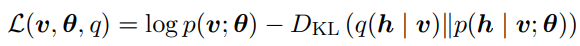
\includegraphics[scale=0.8]{images/ELBO.png}
\end{center}
where $q$ is an arbitrary probability distribution over $\textbf{h}$. The two terms are equal if and only if $q$ is the same distribution as $p(\textbf{h} | \textbf{v})$. We can rearrange $\mathcal{L}$ is a more convenient way:
\begin{center}
    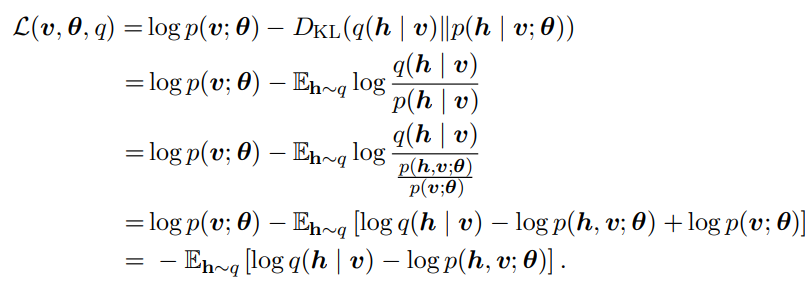
\includegraphics[scale=0.8]{images/ELBO2.png}
    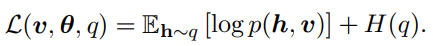
\includegraphics[scale=0.8]{images/ELBO3.png}
\end{center}
When $q(\textbf{h} | \textbf{v})$ = $p(\textbf{h} | \textbf{v})$, the approximation is perfect. We can thus think of inference as the procedure for finding the $q$ that maximizes $\mathcal{L}$.

\section{Differentiable Generator Networks}
Many generative models are based on the idea of using a \textbf{differentiable generator network}. A differentiable generator network transforms samples of latent variables $\textbf{z}$ to samples $\textbf{x}$ (direct) or to distributions over samples $\textbf{x}$ (indirect) using a differentiable function $g(\textbf{z};\theta^{(g)})$, which is typically represented by a neural network. Basically, the idea of differentiable generator networks is to define a distribution over latent variables $\textbf{z}$ (often very simple, like Gaussian distribution), and then learn, via $g$, how to transform the shape of that distribution into the distribution of our training data.\newline\newline
This model class includes variational autoencoders, which pair the generator net with an inference net, generative adversarial networks, which pair the generator network with a discriminator network, and techniques that train generator networks in isolation.\newline\newline
Generator networks are essentially just parametrized computational procedures for generating samples, where the architecture provides the family of possible distributions to sample from and the parameters select a distribution from within that family.\newline\newline
\textbf{Example of direct sample generation:} As an example, the standard procedure for drawing samples from a normal distribution with mean $\mu$ and covariance $\Sigma$ is to feed samples $\textbf{z}$ from a normal distribution with zero mean and identity covariance into a very simple generator network. This generator network contains just one affine layer:
\[\textbf{x} = g(\textbf{z}) = \mu + \textbf{L}\textbf{z}\]
where $\textbf{L}$ is given by the Cholesky decomposition of $\Sigma$.\newline\newline
\textbf{Example of indirect sample generation (define distribution over samples):} Use $g(\cdot)$ with sigmoid outputs to provide the mean parameters of
Bernoulli distributions:
\[p(x_i = 1 | \textbf{z}) = g(\textbf{z})_i\]
we impose a distribution over $\textbf{x}$ by marginalizing $\textbf{z}$:
\[p(\textbf{x}) = \mathbb{E}_\textbf{z}p(\textbf{x}|\textbf{z})\]
As the name suggests, a Differentiable Generator Networks must be differentiable in order to perform gradient-based optimization. However, the sampling from the distribution defined over latent variables $\textbf{z}$
\[z \sim \mathcal{N}(\mu, \sigma^2)\]
is not performed by a function, but it is a stochastic process which changes every time we query it. Therefore, it does not make sense to compute the gradient of $z$ with respect to the parameters of its distribution, $\mu$ and $\sigma^2$. So, we can rewrite the sampling process as transforming an underlying random value $\epsilon \sim \mathcal{N}(\epsilon, 0, 1)$ to obtain a sample from the desired distribution:
\[z = \mu + \sigma \epsilon\]
We are now able to back-propagate through the sampling operation, by regarding it as a deterministic operation with an extra input $\epsilon$. This technique is known as \textbf{reparametrization trick} (this will be more clear when talking about Variational Autoencoders, since in that case $\mu$ and $\sigma$ are parameters that have to be learned).

\section{Variational Autoencoders (VAEs)}
The variational autoencoder is a \textbf{directed model} that uses learned approximate inference and can be trained purely with gradient-based methods.\newline\newline
VAEs assume that our training data $\mathcal{T} = \{\textbf{x}^{(i)}\}^n_{i=1}$ is generated by some latent variables $\textbf{z}$. Let $p_{\theta}(\textbf{z})$ the prior distribution over $\textbf{z}$. The basic idea of VAEs is to set a simple distribution for $p_{\theta}(\textbf{z})$, e.g. Gaussian, and sample $\textbf{z}$ from it. Then, we can use a generator network $g(\textbf{z})$ to estimate $p_{\theta}(\textbf{x}|\textbf{z})$ and generate new samples. The goal is to estimate the parameters $\theta$ of this generative model, that is, how to map $\textbf{x}$ to $\textbf{z}$ and $\textbf{z}$ to $\textbf{x}$. However, both the terms $p_{\theta}(\textbf{x})$ and $p_{\theta}(\textbf{z}|\textbf{x})$ are intractable, so we cannot perform maximum likelihood estimation.\newline\newline
In order to overcome this problem, we can define in addition to the decoder modeling $p_\theta(\textbf{x}|\textbf{z})$ an encoder $q_\phi(\textbf{z}|\textbf{x})$ that approximates $p_\theta(\textbf{z}|\textbf{x})$ using ELBO.
\newline\newline
This lower bound $\mathcal{L}(q)$ is defined as follows:
\begin{center}
    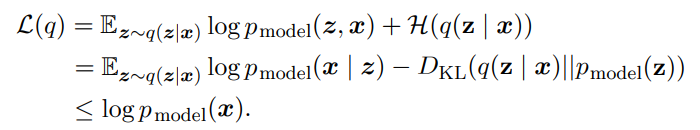
\includegraphics[scale=0.8]{images/VAE.png}
\end{center}
The first term $log\,p_{model}(\textbf{x}|\textbf{z})$ maximizes the likelihood of the original input being reconstructed. The second term $D_{KL}(q(\textbf{z}|\textbf{x}) || p_{model}(\textbf{z}))$ forces the encoder $q_\phi(\textbf{z}|\textbf{x})$ to become a Gaussian prior on $\textbf{z}$ (if we set $p_{\theta}(\textbf{z})$ as a Gaussian). The learning process aims at finding the parameters $\theta^*$, $\phi^*$ for the decoder and encoder that maximize the lower bound.\newline\newline
In other words, the encoder network generates, for each input, two vectors $\mu, \sigma$ representing the mean and the variance of the Gaussian distribution we defined over $\textbf{z}$ (remember that we assumed that the latent variables were distributed according to a Gaussian distribution of 0 mean and variance 1). Then, the decoder network samples from the distribution defined by $\mu$ and $\sigma$, using the \textbf{reparametrization trick}, and performs the reconstruction (remember that we assumed that our data are generated by the latent variables).
\begin{center}
    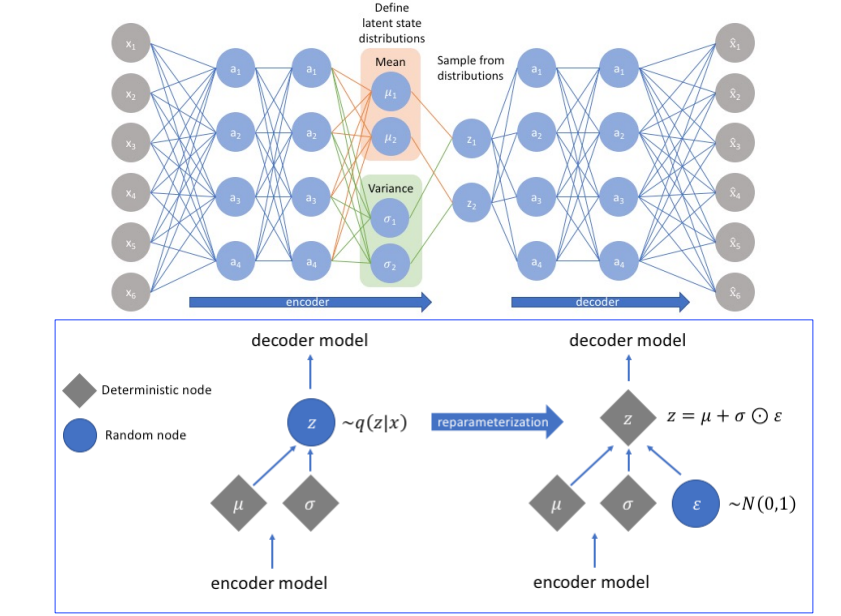
\includegraphics[scale=0.8]{images/VAE2.png}
\end{center}
The reparametrization trick, as we said before, allows the model to learn the parameter related to the mean and variance vectors while maintaining the stochasticity of the entire system via epsilon.\newline\newline 
To generate a sample from the model, the VAE first draws a sample $z$ from the distribution we defined over the latent variables $\textbf{z}$ (Gaussian with mean 0 and variance 1). The sample is then run through a differentiable generator network $g(\textbf{z})$, that is, the decoder. Finally, $\textbf{x}$ is sampled from a distribution $p_{\theta}(\textbf{x}|\textbf{z})$. We usually choose a Gaussian distribution for $p_{\theta}(\textbf{z})$ because is easy to sample from.\newline\newline
The VAE framework is very straightforward to extend to a wide range of model
architectures. One particularly sophisticated VAE is the \textbf{deep recurrent attention writer} or DRAW model. DRAW uses a recurrent encoder and recurrent decoder combined with an attention mechanism. The generation process for the DRAW model consists of sequentially visiting different small image patches and drawing the values of the pixels at those points.

\section{Generative Adversarial Networks (GANs)}
Generative adversarial networks or GANs are another generative modeling approach based on differentiable generator networks.\newline\newline
Generative adversarial networks are based on a game theoretic scenario in which the generator network must compete against an adversary. The generator network directly produces samples $\textbf{x} = g(\textbf{z}; \theta^{(g)})$. Its adversary, the \textbf{discriminator network}, attempts to distinguish between samples drawn from the training data and samples drawn from the generator. The discriminator emits a probability value given by $d(\textbf{x}; \theta^{(d)})$, indicating the probability that $\textbf{x}$ is a real training example rather than a fake sample drawn from the model.\newline\newline
This drives the discriminator to attempt to learn to correctly classify samples as real or fake. Simultaneously, the generator attempts to fool the classifier into believing its samples are real. At convergence, the generator’s samples are indistinguishable from real data, and the discriminator outputs $\frac{1}{2}$ everywhere. The discriminator may then be discarded.\newline\newline
During training, the model samples from a simple distribution, e.g. random noise, and learn a transformation (generator network) to the training distribution. The transformation should be complex enough (e.g. deep neural network).\newline\newline
The objective function is defined as a \textbf{minmax objective function}:
\begin{center}
    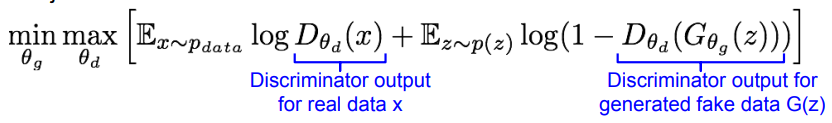
\includegraphics[scale=0.6]{images/GAN.png}
\end{center}
The intuition behind this is that the discriminator network tries to maximize the \textit{accuracy} in determining whether an example is real or fake, while the generator network tries to minimize the performance of the discriminator. If the generator fails to fool the discriminator, it will be punished and it will adapt the generation of new samples accordingly.\newline\newline
In particular, the first term of the function is maximized when the discriminator successfully detects a real image, while the second term is maximized if the generator fails to fool the discriminator (remember that the discriminator outputs a value between 0 and 1 determining the likelihood of a real image).\newline\newline
The training procedure alternates a gradient ascent step on the discriminator, and a gradient descent step on the generator.
\begin{center}
    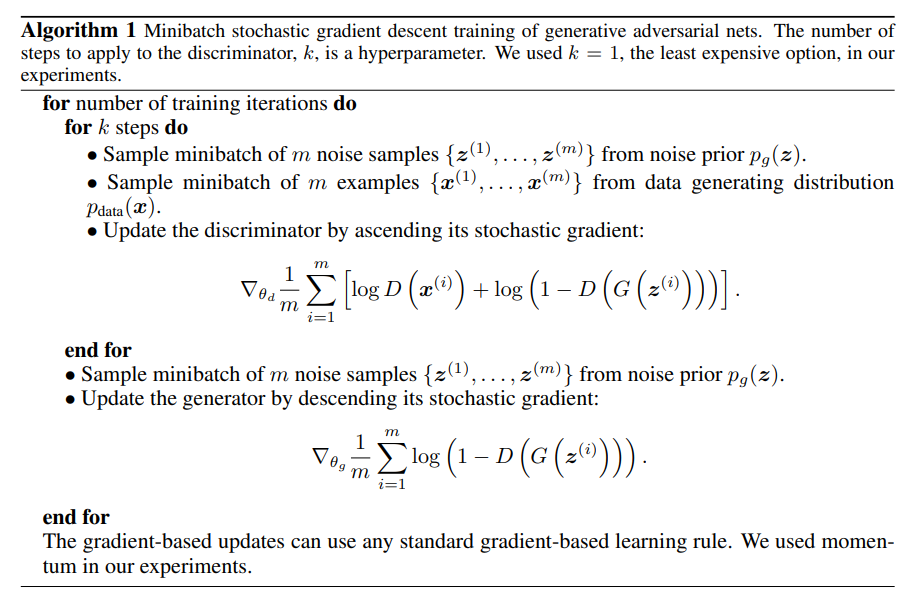
\includegraphics[scale=0.8]{images/training GANs.png}
\end{center}
It can be shown that, under some conditions, eventually the generator converges to the distribution of training data.\newline\newline
The shape of the generator's cost function:
\[log\, (1 - D_{\theta_d}(G_{\theta_g}(z))\]
shows that the generator aims at decreasing the log probability that the discriminator makes the correct prediction. However, we can see that when the generator's samples are likely fake the gradient is small in module, while when the samples fool the discriminator the gradient is large. This is not good for learning, since we want to improve the model when it does not fool the discriminator, and not viceversa.
\begin{center}
    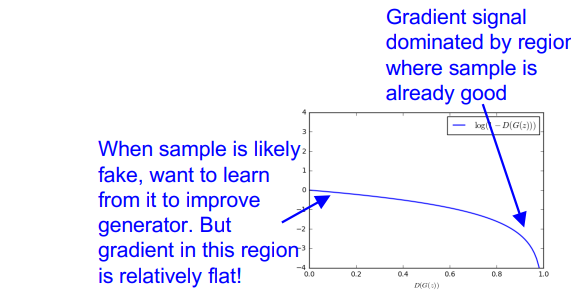
\includegraphics[scale=0.6]{images/GAN2.png}
\end{center}
Therefore, in order to overcome this problem, we can reformulate the objective function such that the generator aims to increase the log probability
that the discriminator makes a mistake, rather than aiming to decrease the log
probability that the discriminator makes the correct prediction.

\section{VAEs vs GANs}
The main motivation for the design of GANs is that the learning process
requires neither approximate inference nor approximation of a partition function gradient. Furthermore, they generate higher quality samples compared to VAEs. However, they can be tricky and unstable to train.\newline\newline
VAEs, instead, provide useful latent representation that allows for inference queries. However, samples from variational autoencoders trained on images tend to be somewhat blurry.
